\documentclass[a4paper]{amsart}

%\usepackage[active]{srcltx}
\usepackage[T1]{fontenc}
\usepackage{amssymb,amsmath,dsfont}
\usepackage{subfigure}
\usepackage{dsfont,graphicx}
\usepackage{graphicx,natbib}
\usepackage{url}
%\numberwithin{equation}{section}
\newtheorem{theorem}{Theorem}[section]
\newtheorem{lemma}{Lemma}[section]
\newtheorem{cor}{Corollary}[section]
%\theoremstyle{definition}
\newtheorem{dfn}{Definition}[section]
%\newtheorem{cdtn}{Condition}[section]
%\newtheorem{exm}{Example}[section]
%\theoremstyle{remark}
\newtheorem{rmk}{Remark}[section]
\newtheorem{proposition}{Proposition}[section]
\renewcommand{\a}{\mathbf a}
\renewcommand{\r}{\mathbb R}
\renewcommand{\l}{\mathbb L}
\newcommand{\e}{\varepsilon }
\newcommand{\A}{\alpha}
\newcommand{\vv}{\varphi }
\renewcommand{\A}{\mathcal{A}( \beta, r, L)}
\newcommand{\Tr}{\text{tr}}
\newcommand{\R}{\mathbb{R}}
\newcommand{\abs}[1]{{\left\lvert#1\right\rvert}} %
\newcommand{\deq}{\mathrel{\mathop:} = } % Igaliti d'assignement
\newcommand{\eqd}{= \mathrel{\mathop:} } % Igaliti d'assignement
\newcommand{\paren}[1]{{\left( #1 \right)}} %
\newcommand{\norm}[2]{{\left\lVert #2 \right\rVert}_{#1}}
\newcommand{\Fourier}[1]{\widetilde{#1}}
\newcommand{\N}{\mathbb{N}}

\usepackage{rotating}

\graphicspath{{images/},{results-rho/},{results-rmse/}}

\title[Adaptive estimation of density matrix in QHT]{Adaptive estimation of the
density matrix in quantum homodyne tomography with noisy data}
\author[P. Alquier \& K.Meziani \& G.Peyr\'e]{Pierre Alquier
\\
{\tiny School of Mathematical Sciences, University College Dublin}
\\ \\
Katia Meziani
\\
{\tiny CEREMADE, Universit\'e Paris-Dauphine}
\\ \\
Gabriel Peyr\'e
\\
{\tiny CEREMADE, Universit\'e Paris-Dauphine}
}
\date{}


\begin{document}

\begin{abstract}
    In the framework of noisy quantum homodyne tomography with
    efficiency parameter $1/2 < \eta \leq 1$, we propose an estimator
    of a quantum state whose density matrix elements $\rho_{m,n}$
    decrease like $Ce^{-B(m+n)^{ r/ 2}}$, for fixed $C\geq 1$, $B>0$ and
    $0<r\leq 2$. On the contrary to previous works, we focus on the
    case where $r$, $C$ and $B$ are unknown. The procedure estimates
    the matrix coefficients by a projection method on the pattern functions,
    following \cite{ABM}, and then by soft-thresholding the coefficients. We
    compute the convergence rates of these estimators, in $\mathbb{L}_2$ risk.
    We obtain the same rate of convergence as if $r$, $C$ and $B$ were known.
\end{abstract}

\maketitle

\tableofcontents


%%%%%%%%%%%%%
\section{Introduction}
%%%%%%%%%%%%%


This paper deals with a \textit{severely ill-posed inverse problem}  come from
quantum optics. 
Quantum optics is a branch of quantum mechanics which studies  physical systems
at the atomic and subatomic scales. As the language used by physicists differs
from the one that used by statisticians, we start with general notions on
quantum mechanics. %(e.g. they speak about "states" or "observables" instead of
"laws" or " random variables"...),
The interested reader can get further acquaintance with quantum  concepts
through the
textbooks  or the review article
\cite{Helstrom,Holevo,Barndorff-Nielsen&Gill&Jupp,Leonhardt}. 



%%%%%%%%%%%%%%%%%%%
\subsection{Physical background}
\label{physbackground}
\noindent\\
%%%%%%%%%%%%%%%%%%


%%%%%%%%%%%%%%%%%%%
\subsubsection{Quantum mechanics}
\label{Quantum mechanics}
\noindent\\
%%%%%%%%%%%%%%%%%%

In quantum mechanics, the quantum state of a system is a mathematical object 
which encompasses all the information about the system.  The most common
representation of a quantum state is an operator $\rho$ on a complex Hilbert
space $\mathcal{H}$ (called the space of states) such that $\rho$ is  
 % 
\begin{enumerate}
     \item Self adjoint: $\rho=\rho^{*}$, where $\rho^{*}$ is the adjoint of
$\rho$.
     \item Positive: $\rho\geq 0$, or equivalently
$\langle\psi,\rho\psi\rangle\geq0$ for all 
               $\psi\in \mathcal  {H}$.
     \item Trace one: $\Tr(\rho)=1$.
\end{enumerate}
A quantum state $\rho$ encodes the probabilities of the measurable properties,
or "\textbf{observables}" (energy, position, ...) of the considered quantum
system. Generally, in quantum mechanics the expected results of the measurements
of an observable are not  deterministic values but  predictions about
probability distributions, that is the probability of obtaining each of the
possible outcomes when measuring an observable. \\
An observable $\mathbf{X}$ is described by a self adjoint operator on the space
of states $\mathcal{H}$ and
$$
\mathbf{X}=\sum_{a}^{dim\mathcal{H}}x_a\mathbf{P}_a,
$$
where the eigenvalues $\{x_a\}_a$ of the observable $\mathbf{X}$ are real and 
$\mathbf{P}_a$  is the projection onto the one dimensional space generated by
the eigenvector of $\mathbf{X}$. Then, when performing a measurement of the
observable $\mathbf{X}$ of a quantum state $\rho$, the result is a random
variable $X$ with values in the set of the eigenvalues of the observable
$\mathbf{X}$. For a quantum system prepared in state $\rho$,  $X$ has the
following probability distribution and expectation  function
%
\begin{center}
$\mathbb{P}_\rho(X=x_a)=Tr(\mathbf{P}_a\rho)$ et
$\quad\mathbb{E}_\rho(X)=Tr(\mathbf{X}\rho)$.
\end{center}
%
\noindent\\
 An important element which affects the result of the measurement process is the
purity of quantum states. A state is called pure if it cannot be represented as
a mixture (convex combination) of other states, i.e., if it is an extreme point
of the convex set of states. All other states are called mixed states. We give
examples of states in Section~\ref{sec.simulations}.



%%%%%%%%%%%%%%%%%%%
\subsubsection{Quantum optics}
\label{Quantum opticcs}
\noindent\\
%%%%%%%%%%%%%%%%%%

In this paper, the quantum system we work with is a monochromatic light in a
cavity described by a quantum harmonic oscillator. In the framework of quantum
optics,  the space of states is known to be the separable Hilbert space
$\mathcal{H}=\mathbb{L}_2(\mathbb{R})$, i.e. the space of square integrable
complex valued functions on the real line. A particular orthonormal basis
$\left(\psi_j\right)_{j\in\mathbb{N}}$ comes with, called the Fock basis. This
physically very meaningful basis is defined for all $j\in\mathbb{N}$ as follow
          \begin{equation}
          \label{eq:fock}
          \psi_j(x)\deq \frac{1}{\sqrt{\sqrt{\pi}2^jj!}}H_j(x)e^{-x^2/2},
          \end{equation}
where $H_j(x) \deq (-1)^j e^{x^2} \frac{d^j}{dx^j} e^{-x^2}$ is the $j$-th
Hermite polynomial. In the Fock basis~\eqref{eq:fock}, a state is described  by
infinite density matrix $\rho=[\rho_{j,k}]_{j,k\in\N}$. \\


We may give  an equivalent  representation for a quantum state $\rho$:  the
associated Wigner function $W_\rho$ (see \cite{Wigner}). The Wigner function
$W_\rho$  is a real function of two variables and may be defined by its Fourier
Transform $\mathcal{F}_2$ with respect to both variables
        \begin{eqnarray*}
         \label{def.Wigner}        
\widetilde{W}_{\rho}(u,v)&:=&\mathcal{F}_2[W_\rho](u,v)=\text{Tr}
\left(\rho\exp(iu\textbf{Q}+iv        
         \textbf{P})\right),
         \end{eqnarray*}
where $\textbf{Q}$ and $\textbf{P}$ are respectively the electric and magnetic
fields.  These two observables, we are concerned by, do not commute. As
non-commuting observables,  they may not be simultaneously measurable. Therefore,
by performing measurements on $(\textbf{Q},\textbf{P})$, we cannot get a density
probability of the result $(Q,P)$.  However, for $\phi\in[0,\pi]$ we can measure
the quadrature observables $\mathbf{X}_\phi :=\mathbf{Q}\cos \phi
+\mathbf{P}\sin \phi$, and then the above Wigner function plays the role of a
quasi-probability density. It does not satisfy all the properties of a
conventional probability distribution but satisfies boundedness properties
unavailable to classical distributions. For instance, the Wigner distribution
can and normally does go negative for states which have no classical model. The
Wigner function is such that
%        
        \begin{itemize}
        \item $W_\rho:\mathbb{R}^2\rightarrow\mathbb{R}$
        \item $\iint_{\R^2} W_\rho(q,p)dqdp=1$,
        \end{itemize}
%        
 However its Radon transform is always a probability density
 %
        \begin{equation}
        \label{eq.Radon.transform}
         p_\rho(x|\phi)   \deq
\mathcal{R}[W_{\rho}](x,\phi)=\int_{-\infty}^\infty W_{\rho}(
        x\cos\phi - t\sin\phi, \, x \sin\phi + t\cos\phi )dt,
         \end{equation}
%         
with respect to $\frac{1}{\pi}\lambda$, $\lambda$ being the Lebesgue measure on
$\mathbb{R}\times [0,\pi]$. 

 
\bigskip


Now we can explicit the links between the state $\rho$ and  the Radon transform
of its associated Wigner function $W_{\rho}$, $p_\rho(x|\phi)$.  In the Fock
basis \eqref{eq:fock}, a state is described  by infinite density matrices
$\rho=[\rho_{j,k}]_{j,k\in\N}$ with entries $\rho_{j,k}$  expressed  as  
       \begin{eqnarray}
       \label{rhojk}
       \rho_{j,k}=\frac 1\pi\int \int_0^\pi
p_\rho(x|\phi)f_{j,k}(x)e^{-i(k-j)\phi}d\phi dx
       \end{eqnarray}
for all $j,k \in\N$.  The functions $f_{j,k} = f_{k,j}$, in the expression
\eqref{rhojk}, are bounded real functions commonly called \textit{pattern
functions} in quantum homodyne literature. A concrete expression for their
Fourier transform using Laguerre polynomials can be found in \cite{Richter1}:
for $j \geq k$,
        \begin{eqnarray}
         \label{Rpattern}
         \tilde{f}_{k,j}(t)  &=&\pi(-i)^{j-k}\sqrt{\frac{2^{k-j} k!}{j!}}|t|
          t^{j-k}e^{-\frac{t^2}{4}}L^{j-k}_k(\frac{t^2}{2}).
         \end{eqnarray}
where $\tilde{f}_{k,j}$ denotes the Fourier transform of the Pattern function
$f_{k,j}$ and 
$$L_{n}^{\alpha}(x) \deq (n!)^{-1} e^x x^{-\alpha} \frac{d^n}{dx^n}
(e^{-x} x^{n+\alpha})$$
 is the Laguerre polynomial of degree $n$ and
order $\alpha$. 




%%%%%%%%%%%%%%%
\subsubsection{QHT}
\label{QHT}
\noindent\\
%%%%%%%%%%%%%%%


 In this paper, we address the problem of reconstructing the density matrix
$\rho$  of a monochromatic light in a cavity.  As the observables $\mathbf{Q}$
and $\mathbf{P}$ cannot  be measured simultaneously,  we measure the quadrature 
$\mathbf{X}_\phi :=\mathbf{Q}\cos \phi +\mathbf{P}\sin \phi$, where
$\phi\in[0,\pi]$. Each of these quadrature could be measured on a laser beam by
a technique put in practice for the first time in \cite{Smithey} and called
Quantum Homodyne Tomography (QHT). The theoretical foundation of quantum
homodyne tomography was outlined in \cite{Vogel&Risken}.




The experimental set-up described in Figure~\ref{Pfig:1} consists of mixing the
cavity pulse prepared in state $\rho$ with an additional laser of high intensity
$\left|z\right|>>1$ called the local oscillator.
 After the mixing, the beam is split again and each of the two emerging beams is
measured by  one of the two photodetectors which give integrated currents $I_1$,
$I_2$ proportional to the number of photons. The result of the measurement is
produced by taking the difference of the two currents and rescaling it by the
intensity $|z|$.  Just before the mixing the experimentalist may choose the
phase $\Phi$ of the local oscillator, randomly, uniformly distributed on
$[0,\pi]$.  In the case of noiseless measurement and for a phase $\Phi=\phi$,
the result $X_\phi=\frac{I_2-I_1}{|z|}$ has density $p_\rho(x|\phi)$
corresponding to measuring $\mathbf{X}_\phi$ . \\


In practice, a number of photons fails to be detected. These losses may be
quantified by one single coefficient $\eta\in[0,1]$, such that  $\eta=0$ when
there is no detection and  $\eta=1$  corresponds to the ideal case. The
physicists argue, that their machines actually have high detection efficiency,
around 0.8/0.9. Thus, we suppose $\eta$ known. As the detection process is
inefficient, an independent gaussian noise interferes additively with the ideal
data $X_\phi$. Thus for $\Phi=\phi$, the effective result of the QHT measurement
(Figure~\ref{Pfig:1}) is   for a known efficiency $\eta\in]0.5,1]$,  
$$
Y=\sqrt{\eta}X_\phi+\sqrt{(1-\eta)/2}\xi
$$
where $\xi$ is a standard Gaussian random variable, independent of $X_\phi$.
%
\begin{figure}[!h]
\begin{center}
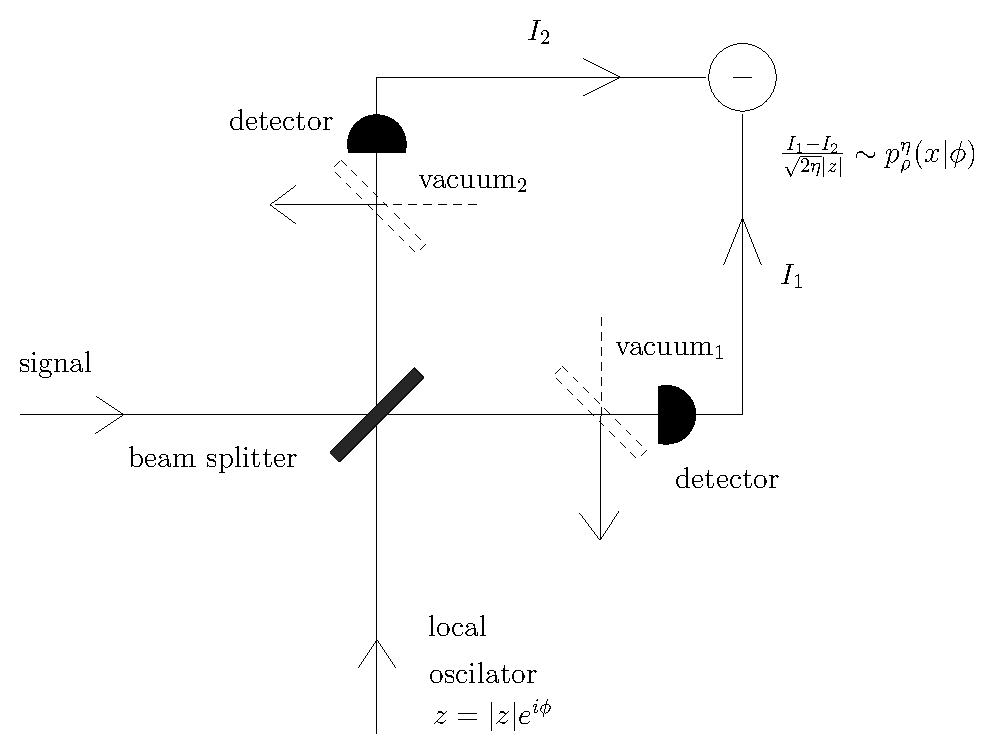
\includegraphics[width=10cm,height=6cm]{noisyQHTsetup.eps}
\caption{QHT measurement scheme}
\label{Pfig:1}
\end{center}
\end{figure}







%%%%%%%%%%%%%%%%%%
\subsection{Statistical model}
\label{Statistical.model}
\noindent\\
%%%%%%%%%%%%%%%%%%

This paper aims at  reconstructing the density matrix of  a monochromatic light
in a cavity prepared in state $\rho$. As we cannot measure precisely the quantum
state in a single experiment, we perform measurements on $n$ independent
identically prepared quantum systems. The measurement
carried out on each of the $n$ systems in state $\rho$ is done by QHT as
described in Section~\ref{QHT}. In the ideal setting, the results of such
experiments would be $n$  independent identically
distributed random variables $(X_{1}, \Phi_{1}),\dots ,(X_{n}, \Phi_{n})$  with
values in $\mathbb{R}\times [0,\pi]$ and distribution $P_{\rho}$ having density 
with respect to $\lambda$, $\lambda$ being the Lebesgue measure on
$\mathbb{R}\times [0,\pi]$ equals to
%
      \begin{equation}
      \label{eq:prhophi}
     p_{\rho}(x,\phi)=\frac 1\pi   p_{\rho}(x|\phi) =\frac 1\pi
\mathcal{R}[W_{\rho}] (x,\phi),
       \end{equation}
%    
where $\mathcal{R}$ is the Radon transform defined in equation
(\ref{eq.Radon.transform}).
As underlined in Section~\ref{QHT},  we do not observe $(X_{\ell},
\Phi_{\ell})_{\ell=1,\ldots n}$ but the noisy version $(Y_{\ell},
\Phi_{\ell})_{\ell=1,\ldots n}$  where
%
      \begin{equation}
      \label{noisy.data}
       Y_\ell:=\sqrt{\eta}X_\ell+\sqrt{(1-\eta)/2}~\xi_\ell.
      \end{equation}
%
Here $\xi_\ell$ are independent standard Gaussian random variables, independent
of all $(X_{\ell}, \Phi_{\ell})$, $\ell=1,\ldots n$. The detection efficiency
$\eta\in]0.5,1]$ is a known parameter and $1-\eta$  represents the proportion of
photons which are not detected due to various losses in the measurement process.
\\
%
Let us denote by $p_{\rho}^{\eta}(y,\phi)$ the density of $(Y_{\ell},
\Phi_{\ell})$. Then,  for $\Phi=\phi$, the density $p_{\rho}^{\eta}(\cdot|\phi)$
is the convolution of the density 
$\frac{1}{\sqrt{\eta}}p_\rho(\frac{\cdot}{\sqrt{\eta}}| \phi)$ of $\sqrt{\eta}X$
with $N^\eta$ the density of a centered Gaussian density having variance $(1
-\eta)/2$ s.t.
%      
       \begin{equation}
       \label{densitbrui}
        p^\eta_\rho(y|\phi) = \left(\frac{1}{\sqrt\eta}
p_\rho\left(\frac{\cdot}{\sqrt\eta}|\phi\right) \ast N^\eta\right)(y)
        = \int_{-\infty}^\infty \frac{1}{\sqrt{\eta}}
p_\rho\left(\frac{y-x}{\sqrt{\eta}}|\phi
        \right) N^\eta (x)dx.%\nonumber
        \end{equation}
 %       
For $\Phi=\phi$, an useful equation in the Fourier domain, deduced by 
the previous relation \eqref{densitbrui} is
       \begin{equation}
       \label{fourierproun}
       \mathcal{F}_1[\sqrt{\eta}p^\eta_\rho(\cdot\sqrt{\eta}|\phi)](t)
        = \mathcal{F}_1[p_\rho(\cdot|\phi)](t)
        \widetilde{N}^\gamma(t),
       \end{equation}
%       
where $\mathcal{F}_{1} $ denotes the Fourier transform with respect to the first
variable and  $\widetilde{N}^\eta(t)=e{-\frac{1-\eta}{4\eta}}$ is the Fourier
transform of $N^\gamma(x)$, the density of a centered Gaussian density having
variance $(1 -\eta)/2\eta=\gamma$.\\ 

In order  to estimate the element of the density matrix defined in \eqref{rhojk}
from the data  $(Y_{\ell}, \Phi_{\ell})_{\ell=1,\ldots n}$, we define a
realistic class of quantum states $\mathcal{R}(C,B,r)$. For $C\geq 1$, $B>0$ and
$0 < r \leq 2$, the class $\mathcal{R}(C,B,r)$ is defined as follow
%
          \begin{equation}\label{eq.classcoeff}
         \mathcal{R}(C,B,r) \deq \{\rho {\rm \ quantum \ state} :
        |\rho_{m,n} |\leq C \exp(-B (m+n)^{r/2})\}.
        \end{equation}
 %       
Note that the class  $\mathcal{R}(C,B,r)$ has been translated in terms of Wigner
functions in \cite{ABM}, where it has been proved that the fast decay of the
elements of the density matrix implies both rapid decay of the Wigner function
and of its Fourier transform.\\
An useful lemma is the following. 

\begin{lemma}
         \label{biais}
         For $\rho\in\mathcal{R}(C,B,r)$, the set defined in
\eqref{eq.classcoeff}, there exists a $M_0$ s.t. $\forall M\geq M_0$   implies
                    \begin{equation}
                     \label{Katia1}
                     \sum_{j+k> M}\rho_{j,k}^{2} \leq \mathcal{C}
M^{2-\frac{r}{2}} e^{-2BM^{\frac{r}{2}}},
                  \end{equation}
                     where $\mathcal{C}=\frac{2C^2}{Br}.$
\end{lemma}

\begin{proof}
For $\rho\in\mathcal{R}(C,B,r)$, we have by the definition of the class
$\mathcal{R}(C,B,r)$ and by Lemma~3 in \cite{ABM}
                  \begin{eqnarray*}
                  \sum_{j+k> M}\rho_{j,k}^{2}\leq C^2  \sum_{j+k> M}\exp(-2B
(j+k)^{r/2})\leq  \frac{2C^2}{Br} M^{2-\frac{r}{2}} e^{-2BM^{\frac{r}{2}}}.
                 \end{eqnarray*}
\end{proof}
However, on the contrary to previous works, we do not assume here that the
constants $r$, $B$ and $C$ are known. From now on we denote by $\langle \cdot,
\cdot \rangle$ and $\| \cdot \|$ the
usual Euclidean scalar product and norm, while $C(\cdot)$ will denote positive
constants depending on parameters given in the parentheses.



%%%%%%%%%%%%%%%%%%%
\subsection{Outline of the results}
\label{Outline.results}
\noindent\\
%%%%%%%%%%%%%%%%%%



%Our aim is to estimate the element of the density matrix defined
%in\eqref{rhojk} from data.  $\mathcal{R}(C,B,r)$, depending on parameters $C\geq
%1$,$B>0$ and $ 0<r\leq 2$, inwhich the elements of the density matrix decrease
%rapidly. 
%\noindent
%The objective is to estimate the unknown state $\rho$ under the assumption that
%it belongs to the class
%In order  to estimate the element of the density matrix defined in
%\eqref{rhojk} from the data  $(Y_{\ell}, \Phi_{\ell})_{\ell=1,\ldots n}$, we
%define a realistic class of quantum states R(B, r), depending on parametersB > 0
%and 0 < r ? 2, in which the elements of the density matrix decrease rapidly.
%InSection 3.2, we prove that the fast decay of the elements of the density
%matrix implies bothrapid decay of the Wigner function and of its Fourier
%transform, allowing us to translate theclasses R(B, r) in terms of Wigner
%functions. \label{Rpattern}



The goal of this paper is to define an estimators of the density matrix and 
to evaluate its performance in $\mathbb{L}_2$ risk.

The reconstruction of the density from
averages of data has been discussed or studied in
\cite{DAriano.0,DAriano.2,DAriano.3,Artiles&Gill&Guta} for $\eta=1$ (no photon
loss). 
Max-likelihood methods have been studied in
\cite{BDPS,Artiles&Gill&Guta,DMS,Guta} and procedure using adaptive
tomographic kernels to minimize the variance has been proposed in \cite{DP}. The
estimation of the density matrix of a quantum state of light in case of
efficiency parameter $\frac12 < \eta \leq 1$ has been discussed in
\cite{DAriano.1,DMS,DAriano.5} and considered in \cite{Richter} via the pattern
functions for the diagonal elements. For the case $0<\eta <1/2$, see \cite{ABM}.
However, the physicists argue, that their machines actually have high detection
efficiency, around $0.8$/$0.9$. So we do not deal here with values of $\eta$
smaller
than $1/2$.

%\noindent

It is to be noted that the estimator proposed in \cite{ABM} depends on the
knowledge of $B$ and $r$. However, in practice, one will face situations where
one wants to reconstruct a density matrix without assuming the knowledge of
$B$ and $r$. This is known in statistics as ``adaptive estimation.''
In this paper, we tackle the problem of adaptive estimation over the class
of quantum states $\mathcal{R}(C,B,r)$.
Our estimator is actually thresholded version of the estimator in \cite{ABM}.
Namely, in \cite{ABM}, an estimator for each coefficient of the density matrix
is proposed. Here, our estimator reaches adaptation by substituting a soft-thresholded
version
to this estimator. Coefficients thresholding is now a classical tool in
statistics.
It was introduced in a series of papers by Donoho and Johnstone
\cite{DJ94,DJ95,DJKP}
in the context of function estimation via wavelets coefficients. See
\cite{Tsybakov1998} for a nice introduction to thresholding and wavelts, see
also
\cite{cai,Alquier2008a}. These methods were extended to inverse problems
\cite{Dinv,Dinv2,kola,cava1},
see \cite{cava2} for an introduction and a survey of the most recent results.

In Section \ref{sec.dens.mat} we define our thresholded estimator for the
density matrix, and state our main result on adaptation. Namely, we prove that
the estimator reaches the same rate as in \cite{ABM} without knowing $B$, $C$ nor $r$. In
Section \ref{sec.simulations}
we provide some simulation study. Proofs are given in Section \ref{sec.proofs}.

To conclude, we may infer that the performances of this estimator with the
estimator of the Wigner function in Chapter 3 of \cite{Katia} and in \cite{ABM}
are comparable. We obtain polynomial rates for the case $r = 2$ and
intermediate rates for $0 < r < 2$ (faster than any logarithm, but slower than
any polynomial).
%  It is convenient to have methods to estimate directly both representations of
% a quantum state.  
%The estimator of the matrix $\rho$ can be easily projected on the space of
%proper quantum states. 
%On the other hand, we may capture some features of the quantum states more
% easily on the Wigner function, for instance when this function has significant
% negative parts, the fact that the quantum state is non classical.









%%%%%%%%%%%%%%%%%
%%%%%%%%%%%%%%%%%
\section{Density matrix estimation}
\label{sec.dens.mat}
%%%%%%%%%%%%%%%%%
%%%%%%%%%%%%%%%%%

The aim of this part is to estimate the density matrix $\rho$ in the Fock basis
directly from the data $(Y_i,\Phi_i)_{i=1,\ldots,n}$. We construct an estimator
of the density matrix $[\rho_{j,k}]_{j,k}$  from a sample of QHT data. We give
theoretical results for our estimator when the quantum state $\rho$ is in $
\mathcal{R}(C,B,r)$, the class of density matrix with decreasing elements
defined in (\ref{eq.classcoeff}).



%%%%%%%%%%%%%%%%%%%%
\subsection{Adapted pattern functions}
\label{Pattern.functions}
\noindent\\
%%%%%%%%%%%%%%%%%%%%


In order to reconstruct the entries of the density matrix from the noisy
observations $(Y_{\ell}, \Phi_{\ell})$ by a projection type estimator on the
\textit{pattern} functions, we have to adapt the pattern functions as follows. 
From now on, we shall use the notation $\gamma=\gamma(\eta) \deq
\frac{1-\eta}{4\eta}$.  We denote by $f^\eta_{k,j}$ the function which has
the following Fourier transform:
%
     \begin{equation}
      \label{eq:patterneta}
      \tilde{f}^\eta_{k,j}(t) \deq \tilde{f}_{k,j}(t) e^{\gamma t^2},
      \end{equation}
%      
where $ \tilde{f}_{k,j}$ are the pattern functions defined in expression
\eqref{Rpattern}. 

\begin{lemma}
         \label{norm}
         For $\eta\in(1/2,1)$, there exists a positive constant
$C^\eta_{\infty}>0$ s.t.
          \begin{equation}
                         \label{normfeta}
                         \sum_{0\leq j+k\leq M} \|f_{j,k}^{\eta}\|_{\infty}^{2}
\leq C_{\infty}^{\eta} M^{\frac{1}{3}}  e^{8\gamma M},
          \end{equation}
          where $\gamma=(1-\eta)/(4\eta)$ and the $(f_{j,k}^{\eta})_{j,k}$ are
the adapted pattern functions defined in expression \eqref{eq:patterneta}.\\
          There exists a positive constant $C_{\infty}>0$ s.t.
           \begin{equation}
                   \label{normf}
                   \sum_{0\leq j+k\leq M} \|f_{j,k}\|_{\infty}^{2} \leq C_\infty
M^{\frac{10}{3}},
           \end{equation}
          where the $ (f_{j,k})_{j,k}$ are the pattern functions defined in
expression \eqref{Rpattern}.
 \end{lemma}

\begin{proof}  
For the proof of this lemma, we refer to Lemma~4 and Lemma~5 in \cite{ABM}.     
   
\end{proof}

%%%%%%%%%%%%%%%%%%
\subsection{Estimation procedure}
\label{Estimation.procedure}
\noindent\\
%%%%%%%%%%%%%%%%%%


 For $N \deq N(n) \rightarrow \infty$, we define the set of indices
$J(N)\subset\mathbb{N}^2$ as
 \begin{equation}
 \label{eqJ}
J(N)\deq\{(j,k)\in\mathbb{N}^2,0\leq j+k \leq N-1\}.
\end{equation}

 For $N \deq N(n) \rightarrow \infty$, let $ \hat{\rho}^\eta$  be a previous
estimator of $\rho$ defined by  its entries
      \begin{eqnarray}
      \label{estrhojk}
       \hat{\rho}^\eta_{j,k} \deq \left\{
       \begin{array}{ccc}
       \frac{1}{n}
\sum_{\ell=1}^{n}G_{j,k}\paren{\frac{Y_\ell}{\sqrt\eta},\Phi_\ell} &
\forall(j,k)\in J (N),\\
                                                                                
                                               0      & \text{  otherwise, }
       \end{array}\right.
      \end{eqnarray}
%
where  $(G_{j,k})_{j,k}$ are the functions using the pattern functions
in~\eqref{eq:patterneta} and 
%
        \begin{equation}
        \label{Gjk}
         G_{j,k}(x,\phi) \deq f^\eta_{j,k}(x) e^{-i(j-k)\phi}.
         \end{equation}
Note that this procedure estimates the matrix coefficients by a projection
method on the pattern functions and has been introduced by  \cite{ABM}.
To define our final procedure estimation, let us introduce some notation. For
any $x\in\mathbb{R}$, we denote by
$(x)_{+}$ the following quantity
%
      \begin{eqnarray}
      \label{qte+}
     (x)_{+} = \left\{ \begin{array}{ccc}
                  x & \text{, if }x\geq 0\\
                  0 & \text{, otherwise. }
                   \end{array}\right.
     \end{eqnarray}
We denote by ${\rm sgn}(\cdot)$  the sign function, given by, $ \forall x\in\mathbb{R}$, 
      \begin{eqnarray}
      \label{sgn}
         {\rm sgn}(x) = \left\{ \begin{array}{ccc}
                       +1 & \text{  if },x>0,\\
                          0& \text{  if },x=0,\\
                          -1 &  \text{  if },x<0.
                             \end{array} \right.
         \end{eqnarray}
From now, we denote by $\|.\|_{\infty}$ the supremum norm for functions, i.e. for any $f$,
$$\|f\|_{\infty}=\sup_{x\in\mathbb{R}}|f(x)|.$$
%
For $N \deq N(n) \rightarrow \infty$ and for some fixed confidence level
$\varepsilon\in(0,1)$, we define the soft-thresholded estimator
        \begin{eqnarray}
        \label{rho-seuil}
        \tilde{\rho}^{\eta}_{j,k} =  {\rm sgn} (\hat{\rho}_{j,k}^{\eta})
         \left(|\hat{\rho}_{j,k}^{\eta}|- t_{j,k} \right)_{+}, 
        \end{eqnarray}
where
       \begin{equation}
      \label{tjk}
       t_{j,k} = \|f_{j,k}^{\eta}\|_{\infty}\sqrt{\frac{
2\log\left(\frac{N(N+1)}{\varepsilon}\right)}{n}}. 
      \end{equation}
Finally, our density matrix estimator is given by
$$\tilde{\rho}^{\eta}=[\tilde{\rho}^{\eta}_{j,k}]_{j,k} .$$




%%%%%%%%%%%%%
\subsection{Main results}
\label{Main.results}
\noindent\\
%%%%%%%%%%%%%

For any density matrix $\nu=(\nu_{j,k})_{j,k\geq 0}$, we define the
$\ell_{2}$-norm of $\nu$ as
$$
 \|\nu \|_{2} = \sqrt{ \sum_{j,k\geq 0} \nu_{j,k}^{2} } .
 $$
We have the following oracle inequality that will allow to obtain rates of
convergence on the classes $\mathcal{R}(C,B,r)$.


 \begin{theorem}
           \label{thm.oracle}
           With probability larger than
$1-\varepsilon$, we have
           $$
          \left\|\tilde{\rho}^\eta - \rho \right\|^{2}_{2}  \leq
\inf_{I\subseteq J(N)} \left\{ 4 \sum_
            {(j,k)\in I} t_{j,k}^{2} + \sum_{(j,k)\notin I}\rho_{j,k}^{2}
\right\},
           $$
           where the set $J(N)$ is defined in \eqref{eqJ}.
\end{theorem}
The proof is given in Section \ref{sec.proofs}.


\begin{cor}
           \label{coro1}
           Let us put $r_{0}\in(0,2)$, $B_{0}>0$ and let us choose
                    \begin{equation}
         \label{Ncorr1}
                      N = N(n) := \left\lfloor \left(\frac{\log(n)}{2B_{0}}\right)^{\frac{2}{r_{0}}}
                   \right\rfloor,
           \end{equation}
where $\left\lfloor x \right\rfloor$ denote the integer part of $x$ such that $\left\lfloor x \right\rfloor\leq x\leq  \left\lfloor x \right\rfloor+1$. Let us assume that we are in the case $\rho\in\mathcal{R}(C,B,r)$, for some
unknown $C\geq 1$, $B\geq B_{0}$, $r\in[r_0 , 2]$. Then, there are constants
$\mathcal{C}_{1},\mathcal{C}_ {2},\mathcal{C}_{3}>0$ such that with probability
larger than $1-\varepsilon$, we have\\
\begin{itemize}
\item For  $\eta = 1$ and $r\in[r_0,2]$
            \begin{align*}
                    \left\|\tilde{\rho}^\eta - \rho \right\|^{2}_{2}
\leq\mathcal{C}_1 n^{-1}\left(\log(n)\right)^{\frac{20}{3r}}\log
\left(\log(n)/\varepsilon\right).
              \end{align*}      \\
\item   For $\eta\in(\frac{1}{2},1)$ and $ r=2$             
            \begin{align*}
                    \left\|\tilde{\rho}^\eta - \rho \right\|^{2}_{2}\leq
\mathcal{C}_2   n^{-\frac{B}{4\gamma+B}}\left(\log(n)+\left(\log(n)\right)^{1/3}
\log\left( \log (n)/\varepsilon\right) \right). 
            \end{align*} \\               
\item   For $\eta\in(\frac{1}{2},1)$ and  $r\in(r_0,2)$                
            \begin{align*}
                    \left\|\tilde{\rho}^\eta - \rho \right\|^{2}_{2}\leq 
\mathcal{C}_3   e^{-2BM(n)^{r/2}} \left( \log(n)^{2-r/2}
+\log(n)^{1/3}\log\left( \log (n)/\varepsilon\right)  \right),
                   \end{align*} \\
 where $ M(n) $ satisfies $8 \gamma M(n) + 2 B M(n)^{r/2} = \log(n)$.  In
particular, note that 
 $$ M(n)= \frac{1}{8\gamma} \log(n) - \frac{2B}{(8\gamma)^{1+r/2}} \log(n)^{r/2}
+ o(\log(n)^{r/2}).$$
 \end{itemize}
\end{cor}
The rate of convergence in the case $1>\eta>\frac{1}{2}$ and $r_{0}<r<2$ is
slower than any polynomial rate but faster than any logarithmic rate.
Observe that we obtain exactly the same rate than in \cite{ABM} and
\cite{Katia}, up to a $\log(\log(n)/\varepsilon)$ term. But on the other hand,
this result is adaptive, in the sense that we do not have to know $B$ or $r$ to
build the estimator.

%%%%%%%%%%%%%%%%%%begin proof cor1
\begin{proof}[Proof of Corollary \ref{coro1}]
For $r_{0}\in(0,2)$, $B_{0}>0$ and $N$ as in \eqref{Ncorr1}, let $M$ be an integer s.t. $M<N$. We define the set 
$$J(M) := \{(j,k)\in \mathbb{N}^2,\, 0\leq j+k\leq M\}.$$
 Then, for $\varepsilon\in (0,1)$ and by applying Theorem \ref{thm.oracle} to $I
= J(M)$, with probability larger than $1-\varepsilon$, we obtain
       \begin{align}
               \nonumber
                \left\|\tilde{\rho}^\eta - \rho \right\|^{2}_{2} 
                & \leq \inf_{0\leq M \leq N-1}\left\{ 4 \sum_{0\leq j+k\leq M}
t_{j,k}^{2} + \sum_{j+k> M}\rho_{j,k}^{2}  \right\} \\
                & = \inf_{0\leq M \leq N-1}\left\{ \frac{8}{n} \sum_{0\leq
j+k\leq M} \|f_{j,k}^\eta\|_{\infty}^{2}\log\left(N(N+1)/\varepsilon\right)+
\sum_{j+k> M}\rho_{j,k}^{2} \right\}.
             \label{etape1}
     \end{align}
 \noindent\\
     
%%%%%%%%%%%%%%%%%%
\paragraph{\textit{a) For $\eta=1$ and $r\in[r_0,2]$.}}
\noindent\\
%%%%%%%%%

 %
As  $ f_{j,k}^\eta=f_{j,k}$ for $\eta=1$, we have by pluging  \eqref{Katia1} and
\eqref{normf} into \eqref{etape1} 
       \begin{align}
               \nonumber
                \left\|\tilde{\rho}^\eta - \rho \right\|^{2}_{2} 
                & \leq \inf_{0\leq M \leq N-1}\left\{ \frac{8}{n} \sum_{0\leq
j+k\leq M} \|f_{j,k}\|_{\infty}^{2}\log\left(N(N+1)/\varepsilon\right)+
\sum_{j+k> M}\rho_{j,k}^{2} \right\}.
                 \nonumber\\
                 &\leq \inf_{0\leq M \leq N-1}\left\{\frac{c_1}{n}
M^{\frac{10}{3}}\log(N/\varepsilon)  + \mathcal{C} M^{2-\frac{r}{2}}
e^{-2BM^{\frac{r}{2}}} \right\},
 \label{etape2}
     \end{align}
for some constant $c_1>0$.\\
 For $N$ such in \eqref{Ncorr1} and by taking $M=(\log(n)/2B)^{2/r}<N$, it leads
to
$$
 \left\|\tilde{\rho}^\eta  - \rho \right\|^{2}_{2}  \leq\mathcal{C}_1 \log
\left(\log(n)/\varepsilon\right)
 \left(\log(n)\right)^{\frac{20}{3r}} n^{-1}
$$
for some constant $\mathcal{C}_{1}>0$.
\noindent\\ 


%%%%%%%%%%%%%%%%%%
\paragraph{\textit{b) For $\eta\in(1/2,1)$ and $r=2$.}}
\noindent\\
%%%%%%%%%


%
Next, we deal with the case $1>\eta>1/2$. We plug \eqref{Katia1} and
\eqref{normfeta} into \eqref{etape1} to obtain in the case $r=2$
              \begin{equation*}
                        \left\|\tilde{\rho}^\eta  - \rho \right\|^{2}_{2}
\leq\inf_{0\leq M <N }\left\{ \frac{c_{2}}{n}  \log\left(N/
                        \varepsilon\right)M^{\frac{1}{3}} e^{8 \gamma M}+
\mathcal{C}M  e^{-2BM}\right\},
               \end{equation*}
for some constant $c_2>0$.\\
By taking $M=M(n)$ s.t.
$$ 
M=\frac{\log(n)}{2(4\gamma+B)} ,%\left(1+\frac{2}{3} \frac{\log\log(n)}{\log(n)}
$$
we obtain
$$
 \left\|\tilde{\rho}^\eta - \rho \right\|^{2}_{2}  \leq\mathcal{C}_2  
n^{-\frac{B}{4\gamma+B}}\left(\log\left( \log (n)/\varepsilon\right)
\left(\log(n)\right)^{1/3}+\log(n) \right) ,
$$
for some constant $\mathcal{C}_2 >0$. 
\noindent\\ 

%%%%%%%%%%%%%%%%%%
\paragraph{\textit{c) For $\eta\in(1/2,1)$ and $r\in(r_0,2)$.}}
\noindent\\
%%%%%%%%%
Finally, in the case $\eta\in(1/2,1)$ and $r\in(r_0,2)$ and by plugging 
\eqref{Katia1} and \eqref{normfeta} into \eqref{etape1} we get:
              \begin{equation*}
                        \left\|\tilde{\rho}^\eta  - \rho \right\|^{2}_{2}
\leq\inf_{0\leq M <N }\left\{ \frac{c_3}{n}\log\left(N
                        /\varepsilon\right) M^{\frac{1}{3}} e^{8 \gamma M}+
\mathcal{C} M^{2-\frac{r}{2}}  e^{-2BM^{\frac{r}{2}}}\right\},
               \end{equation*}
%
for some constant $c_3>0$.\\
For $M$ a solution of the equation $8\gamma M +2 B M^{\frac{r}{2}} = \log(n)$
and for 
$$ M(n)= \frac{1}{8\gamma} \log(n) - \frac{2B}{(8\gamma)^{1+r/2}} \log(n)^{r/2}
+ o(\log(n)^{r/2})$$
in particular, we obtain 
$$
 \left\|\tilde{\rho}^\eta - \rho \right\|^{2}_{2}  \leq\mathcal{C}_3  
\exp^{-2BM^{r/2}} \left( \log(n)^{2-r/2} +
 \log(n)^{1/3}\log\left(N/\varepsilon\right) \right),
$$
for some constant $\mathcal{C}_3 >0$. 
\end{proof}
%%%%%%%%%%%%%%%%%%%%%%%%%end proof cor1




Finally, let us remark that in the case where $\rho$ is a pure state, we even
have a faster rate of convergence.

\begin{cor}
 \label{coro2}
              Under the same choice for $N$ than in Corollary \ref{coro1},
              $$
               N = N(n) := \left\lfloor
\left(\frac{\log(n)}{2B_{0}}\right)^{\frac{2}{r_{0}}} \right\rfloor, 
              $$
            if $\rho$ is a pure state, i.e., if $\rho_{j_0,j_0} = 1$ and all the
others $\rho_{j,k}=0$, then we have, as soon as $N> \max(j_{0},2)$, with
probability larger than $1-\varepsilon$, 
              $$
              \left\|\tilde{\rho}^\eta - \rho \right\|^{2}_{2}  < \frac{32}{n
r_0} \|f_{j_0,j_0}\|_{\infty}^2 \log\left(\frac{\log(n)} {B_0
\varepsilon}\right).
              $$
\end{cor}


%%%%%%%%%%%%%%%%%%%%%%begin Proof of Corollary \ref{coro2}
\begin{proof}[Proof of Corollary \ref{coro2}]
We apply Theorem \ref{thm.oracle} for $I = \{(j_0,j_0)\}$. We obtain, with
probability larger than
$1-\varepsilon$,
           \begin{align*}
                      \left\|\tilde{\rho}^\eta - \rho \right\|^{2}_{2}& \leq
\frac{8}{n} \sum_{(j,k)=(j_0,j_0)} \|f_{j,k}\|_{\infty}^{2}
                     \log\left(N(N+1)/\varepsilon\right)+ \sum_{(j,k)\neq
(j_0,j_0)}\rho_{j,k}^{2}  \\
                       & = \frac{8}{n} \|f_{j_0,j_0}\|_{\infty}^{2}
                     \log\left(N(N+1)/\varepsilon\right)+ 0.
           \end{align*}
For $n$ large enough,  $N=N(n)\geq2$. Then, $(N+1)< 2N$ and 
           \begin{align*}
                      \left\|\tilde{\rho}^\eta - \rho \right\|^{2}_{2}& < 
\frac{8}{n} \|f_{j_0,j_0}\|_{\infty}^{2}
                     \log\left(2N^2/\varepsilon\right) \\
                     & = \frac{8}{n} \|f_{j_0,j_0}\|_{\infty}^{2} \left[
                     2 \log(N) + \log\left(2/\varepsilon\right) \right] \\
                     & \leq  \frac{8}{n} \|f_{j_0,j_0}\|_{\infty}^{2} \left[
                     \frac{4}{r_{0}} \log\left(\frac{\log(n)}{2B_{0}}\right) +
\log\left(2/\varepsilon\right) \right]
           \end{align*}
where we replaced $N$ by its definition. As $r_0 < 2$, $4/r_0 > 1$ and we have
the following rough upper bound:
 \begin{align*}
                      \left\|\tilde{\rho}^\eta - \rho \right\|^{2}_{2} & <
\frac{8}{n} \|f_{j_0,j_0}\|_{\infty}^{2} \left[
                     \frac{4}{r_{0}} \log\left(\frac{\log(n)}{2B_{0}}\right) + 
\frac{4}{r_{0}}  \log\left(2/\varepsilon\right) \right] \\
                       & = \frac{32}{nr_{0}} \|f_{j_0,j_0}\|_{\infty}^{2}
\log\left(\frac{\log(n)}{B_{0} \varepsilon}\right).
           \end{align*}
 \end{proof}
%%%%%%%%%%%%%%%%%%%%%end Proof of Corollary \ref{coro2}

%%%%%%%%%%%%%%%%%%
%%%%%%%%%%%%%%%%%%
\section{Simulation study}
\label{sec.simulations}

%%%%%%%%%%%%%%%%%%%%
%%%%%%%%%%%%%%%%%%%%
\subsection{Examples}



\begin{table}[htbp!]
\begin{center}%
\caption{Examples of quantum states}
\label{TTtab:1}
\vspace{.2cm}
\begin{tabular}{|l|}
\hline
\textbf{\textit{Vacuum} state}  \\
$\bullet$ $\rho_{0,0}=1$ rest zero,\\
$\bullet$ $p_\rho(x|\phi)=e^{-x^2}/\sqrt{\pi}$. \\
%
\hline
\textbf{Single photon state}\\
$\bullet$ $\rho_{1,1}=1$ rest zero,\\
$\bullet$ $p_\rho(x|\phi)=2x^2e^{-x^2}/\sqrt{\pi}.$\\
%
\hline
\textbf{\textit{Coherent-$q_0$} state }$q_0\in\mathbb{R}$ \\
$\bullet$ $\rho_{j,k}=e^{-|q_0|^2}(q_0/\sqrt{2})^{j+k}/\sqrt{j!k!}$,\\
$\bullet$ $p_\rho(x|\phi)=\exp(-(x-q_0\cos(\phi))^2)/\sqrt{\pi}.$\\
%
\hline       
%\textbf{\textit{Squeezed state}}  $M\in\mathbb{R}_+$, $\xi\in\mathbb{R}$ \\
%$\bullet$ $\rho_{j,k}=C(M,\xi)(\frac 12
%\tanh(\xi))^{k+j}H_j(\delta)H_k(\delta)/\sqrt{j!k!}$,\\
%$\bullet$
%$p_\rho(x|\phi)=\exp\left[\left(\sin^2(\phi)(xe^{-2\xi}\cos(\phi)-(x\cos(\phi)-
%\alpha)e^{2\xi})^2\right)/\left(e^{2\xi}\sin^2(\phi)+e^{-2\xi}
%\cos^2(\phi)\right) \right.$\\
%$\quad$ $\quad$ $\quad$ $\quad$ $\times\left.-e^{-2\xi}(x\cos(\phi)-
%\alpha)^2-e^{2\xi}x^2\sin^2(\phi)
%\right]/\sqrt{\pi(e^{2\xi}\sin^2(\phi)+e^{-2\xi}\cos^2(\phi))}.$ \\
%
%\hline        
\textbf{\textit{Thermal state}} $\beta>0$\\
$\bullet$ $\rho_{j,k}=\delta^j_k(1-e^{-\beta})e^{-\beta k}$,\\
$\bullet$ $p_\rho(x|\phi)=\sqrt{\tanh(\beta/2)/\pi}\exp(-x^2\tanh(\beta/2)).$\\
%
\hline
\textbf{\textit{Schr\"{o}dinger cat}} $q_0>0$ \\
$\bullet$
$\rho_{j,k}=2(q_0/\sqrt{2})^{j+k}/\left(\sqrt{j!k!}
(\exp(q_0^2/2)+\exp(-q_0^2/2))\right)$, for $j$ and $k$ even, rest zero,\\
$\bullet$ $p_\rho(x|\phi)=\left(\exp(-(x-q_0\cos(\phi))^2)+\exp(-(x+q_0
\cos(\phi))^2)\right.$\\
$ \quad$ $ \quad$ $ \quad$ $ \quad$
$\left.+2\cos(2q_0x\sin(\phi))\exp(-x^2-q_0^2\cos^2(\phi))\right)%$%\\
 %$ \quad$ $ \quad$ $ \quad$ $ \quad$  
 /\left(2\sqrt{\pi}(1+\exp(-q_0^2))\right).$\\
 \hline
\end{tabular}
\end{center}
\end{table}

 %A state is called pure if it cannot be represented as a mixture (convex combination) of other states, i.e., if it is an extreme point of the convex set of states. This is equivalent to the density matrix being a one dimensional projector, i.e., of the form $\rho=\textbf{P}_{\psi}$ for some unit vector $\psi$. In this case the formula for the expectation value of an operator $A$ in the state simplifies as $tr(A\rho)=E_\rho[A]$. Equivalently, a state $\rho$ is pure if $\text{Tr}(\rho^2)=1$. All other states are called mixed states.\\
We present in Table~\ref{TTtab:1} examples of pure quantum states, which can be
created at this moment in laboratory and belong to the class $\mathcal{R}(C,B,r)$ with $r=2$.   Table~\ref{TTtab:1} gives also their explicit density matrix coefficients $\rho_{j,k}$ and probability densities $p_\rho(x|\phi)$.\\
Among the pure states we consider the \textit{vacuum} state, which is the pure state of zero photons. Note that the \textit{vacuum} state would
provide a random variable of Gaussian probability density $p_\rho(x|\phi)$ via the ideal measurement of QHT (see Section~\ref{QHT}). That explains the gaussian nature of the noise in the effective result of the QHT measurement. \\
The \textit{single photon} state, which is the pure state of one photon. We consider also the \textit{coherent-$q_0$} state, which characterizes the laser pulse with the number of photons  Poisson distributed with an average of $M$ photons.
% The \textit{Squeezed} states (see e.g. \cite{Breitenbach&Schiller&Mlynek}) have Gaussian Wigner functions whose variances in the two directions have a fixed product. The parameters $M$ and $\xi$ are such that $M\geq \sinh^2(\xi)$,$C(M,\xi)$ is a normalization constant, $\alpha=\frac{(M-\sinh^2(\xi))^{1/2}}{\cosh(\xi)-\sinh(\xi)}$, and $\delta=\left(\frac{\alpha}{\sinh(2\xi)}\right)^{1/2}$.
Remark that the well-known \textit{Schr\"{o}dinger cat} state is described by a linear
superposition of two \textit{coherent} vectors (see e.g. \cite{Our}).



%%%%%%%%%%%%%%%%%%%%%%
\subsection{Pattern functions $f^\eta_{j,k}$}
\label{TTsimu.pattern.function}
%%%%%%%%%%%%%%%%%%%%%%

Since there is no closed-form expression for the pattern functions $f^\eta_{j,k}$, we evaluate them numerically on a 1-D regular grid of $Q=4096$ points. We use expressions~\eqref{Rpattern} and~\eqref{eq:patterneta} to evaluate $\tilde f_{j,k}$ and $\tilde f_{j,k}^\eta$  on the 1-D frequency grid of $Q$ discretized $t$ points. The adapted pattern functions $f_{j,k}^\eta$ are computed on the 1-D spacial grid of $Q$ discretized $x$ points by applying to $\tilde f_{j,k}^\eta$ the inverse Fast Fourier Transform (FFT) in $O(Q \log(Q))$ operations. Figure~\ref{fig:example-pattern} shows a few examples of pattern functions. 


\begin{figure}[!h]
\begin{center}
\begin{tabular}{@{}c@{\hspace{1mm}}c@{}}
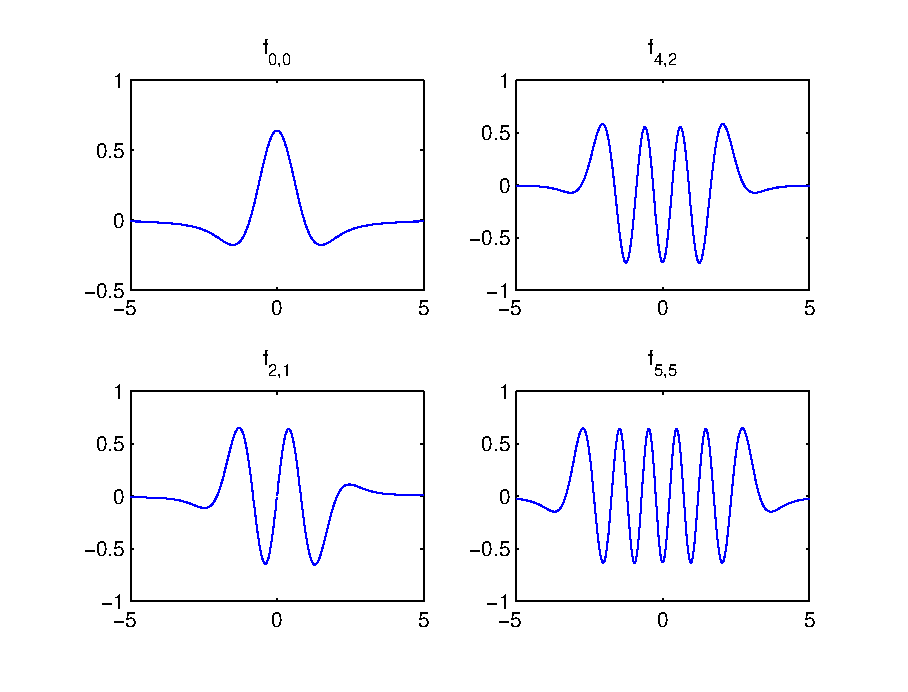
\includegraphics[width=.49\linewidth]{pattern}&
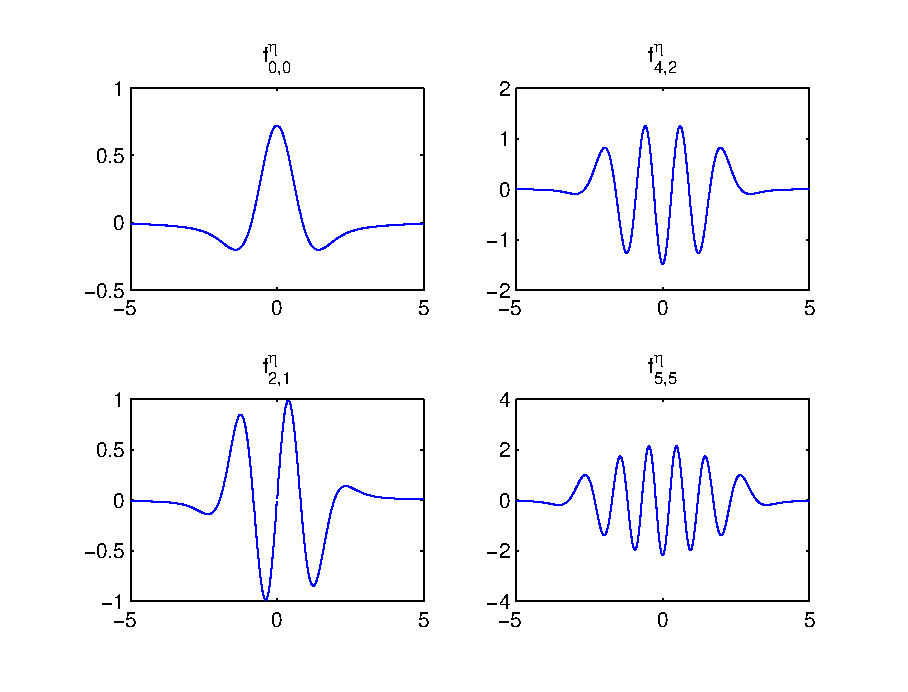
\includegraphics[width=.49\linewidth]{patterneta}\\
\end{tabular}
\caption{ % 
	Examples of pattern functions $f_{j,k}$ (left) and adapted pattern functions $f_{j,k}^\eta$ (right).
}
\label{fig:example-pattern}
\end{center}
\end{figure}



%%%%%%%%%%%%%%%%%%%%%%%
\subsection{Implementation of our procedure}
\label{TTimplementation.Mn}
%%%%%%%%%%%%%%%%%%%%%%%


The deconvolved estimator $\hat{\rho}^\eta_{j,k}$ defined in~\eqref{estrhojk} is computed by evaluating $ G_{j,k}(x,\phi) = f^\eta_{j,k}(x) e^{-i(j-k)\phi}$ at point $x$ using a cubic spline interpolation of the values of $f^\eta_{j,k}$ on the discrete grid of $Q$ points.

In the following section, we evaluate the performance of the threshold estimator $\tilde{\rho}^{\eta}_{j,k}$. We perform this evaluation by creating noisy samples $Y_\ell$ as defined in~\eqref{noisy.data}. The initial samples $X_\ell$ are drawn from the distribution $p_\rho(x | \phi)$ (see Table~\ref{TTtab:1}) using the rejection method. 

The value of $N=N(n)$ is set following~\eqref{Ncorr1}. We use $r_0=2$ and $B_0=1/2$ for all the numerical experiments.

A toolbox that implements this procedure and reproduces all the figures of this article is available online\footnote{\url{http://www.ceremade.dauphine.fr/~peyre/codes/}}.

%%%%%%%%%%%%%%%%%%%%%%%%%%%%%%%
\subsection{Studies of the performance of our test procedure }
\label{TTperformanceOmega}
%%%%%%%%%%%%%%%%%%%%%%%%%%%%%%%



\newcommand{\myfiga}[1]{\includegraphics[width=.32\linewidth]{#1/#1-rho}}
\newcommand{\myfig}[3]{\includegraphics[width=.32\linewidth]{#1/b0-#2/#1-n#3}}
% Change this value to select a different B0=\Bvalue/10 value.
\newcommand{\Bvalue}{5}
\newcommand{\vertText}[1]{ \rotatebox{90}{\mbox{\hspace{1cm} #1}}   }
\begin{figure}[!h]
\begin{center}
\begin{tabular}{@{}c@{\hspace{1mm}}c@{\hspace{1mm}}c@{\hspace{1mm}}c@{}}
\vertText{$\rho$} & \myfiga{coherent}   				&  \myfiga{shrodinger-cat}				&   \myfiga{thermal}					\\
\vertText{$n=10^4$} & \myfig{coherent}{\Bvalue}{10k}	&   \myfig{shrodinger-cat}{\Bvalue}{10k}	&   \myfig{thermal}{\Bvalue}{10k}			\\
\vertText{$n=10^5$} & \myfig{coherent}{\Bvalue}{100k}	&   \myfig{shrodinger-cat}{\Bvalue}{100k}	&   \myfig{thermal}{\Bvalue}{100k}			\\
\vertText{$n=10^6$} & \myfig{coherent}{\Bvalue}{1000k}	&   \myfig{shrodinger-cat}{\Bvalue}{1000k}	&   \myfig{thermal}{\Bvalue}{1000k}	\\
\vertText{$n=10^8$} & \myfig{coherent}{\Bvalue}{100000k}	&   \myfig{shrodinger-cat}{\Bvalue}{100000k}	&   \myfig{thermal}{\Bvalue}{100000k}	\\
    & Coherent $q_0=3$ &
Schr\"{o}dinger cat $q_0=3$ &
Thermal $\beta=1/4$
\end{tabular}
\caption{First row: $\rho$.
  Following rows: estimated $\tilde \rho^\eta$ for $B_0=0.\Bvalue{}$, $\eta=0.9$, $\varepsilon=1$ and $n$ respectively equal to 
  $10^4$ (row \#2), 
  $10^5$ (row \#3), 
  $10^6$ (row \#4), 
  $10^8$ (row \#5). }
\label{fig:examples}
\end{center}
\end{figure}

Figure~\ref{fig:examples} shows graphically the result of our estimator for three different pure quantum states, for several values of $n$. To further evaluate quantitatively the performance of the method, we estimate numerically the (relative) root mean square error (RMSE) 
\begin{equation*}
	\text{RMSE}(n) = \frac{ \| \tilde \rho^\eta - \rho \| }{�\| \rho \| }
\end{equation*}
of our soft thresholding estimator. More precisely, Figure~\ref{fig:RMSE} shows the evolution with $n$ of the expected value of the RMSE. This expected value is evaluated by an empirical mean with Monte Carlo simulation using 50 samplings for each value of $n$. To evaluate the deviation with respect with this mean, we also display the confidence interval at $\pm 3$ times the standard deviation of the RMSE. 

The threshold values $t_{j,k}$ that are used in~\eqref{rho-seuil} to define our estimator are somehow conservative. In practice, smaller values offer better decay of the RMSE. Figure~\eqref{fig:RMSE} display in dashed red (reap. dashed green) the decay of the RMSE obtained using thresholds $0.8 t_{j,k}$ (resp. $0.5 t_{j,k}$). We found on these three examples and for $\eta=0.9$ that using $0.5 t_{j,k}$ gives consistently the lowest RMSE among other choices of thresholds proportional to the $t_{j,k}$ values.

\begin{figure}[!h]
\begin{center}
\begin{tabular}{@{}c@{\hspace{1mm}}c@{}}
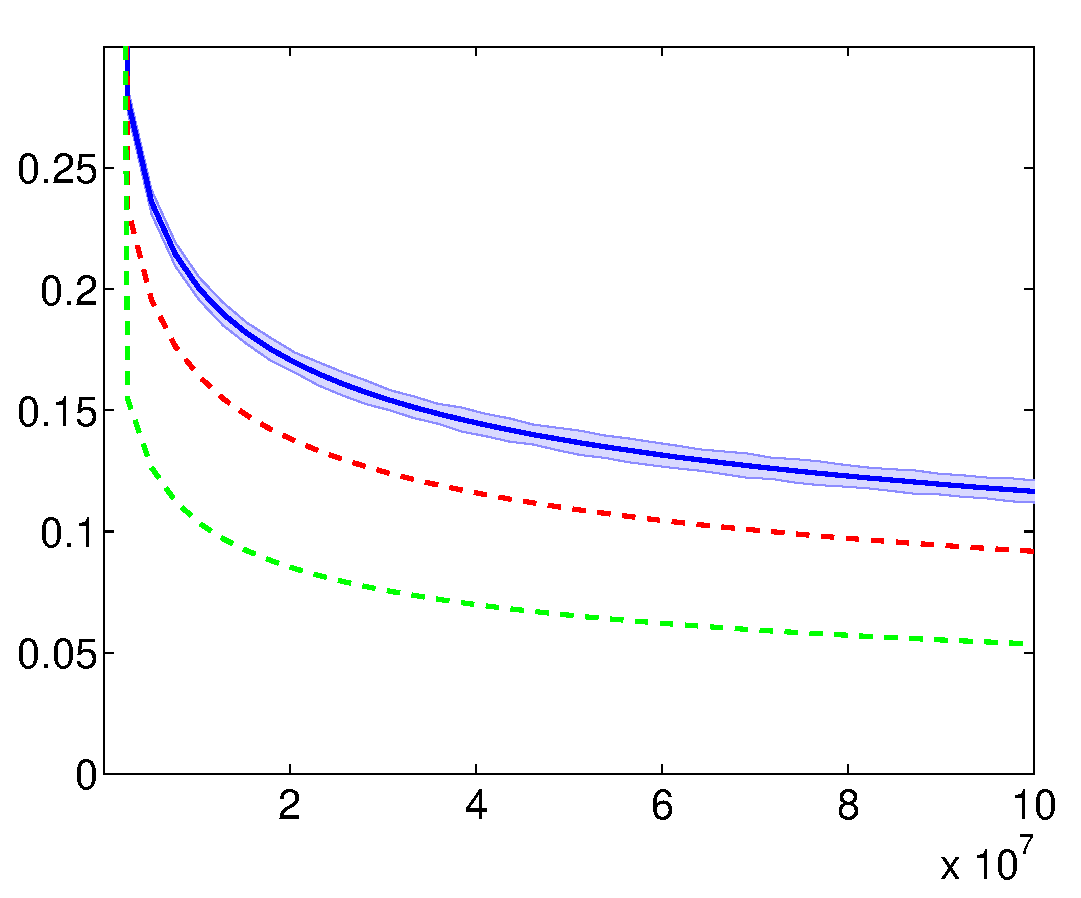
\includegraphics[width=.45\linewidth]{results-rmse/coherent-eta9-rmse}&
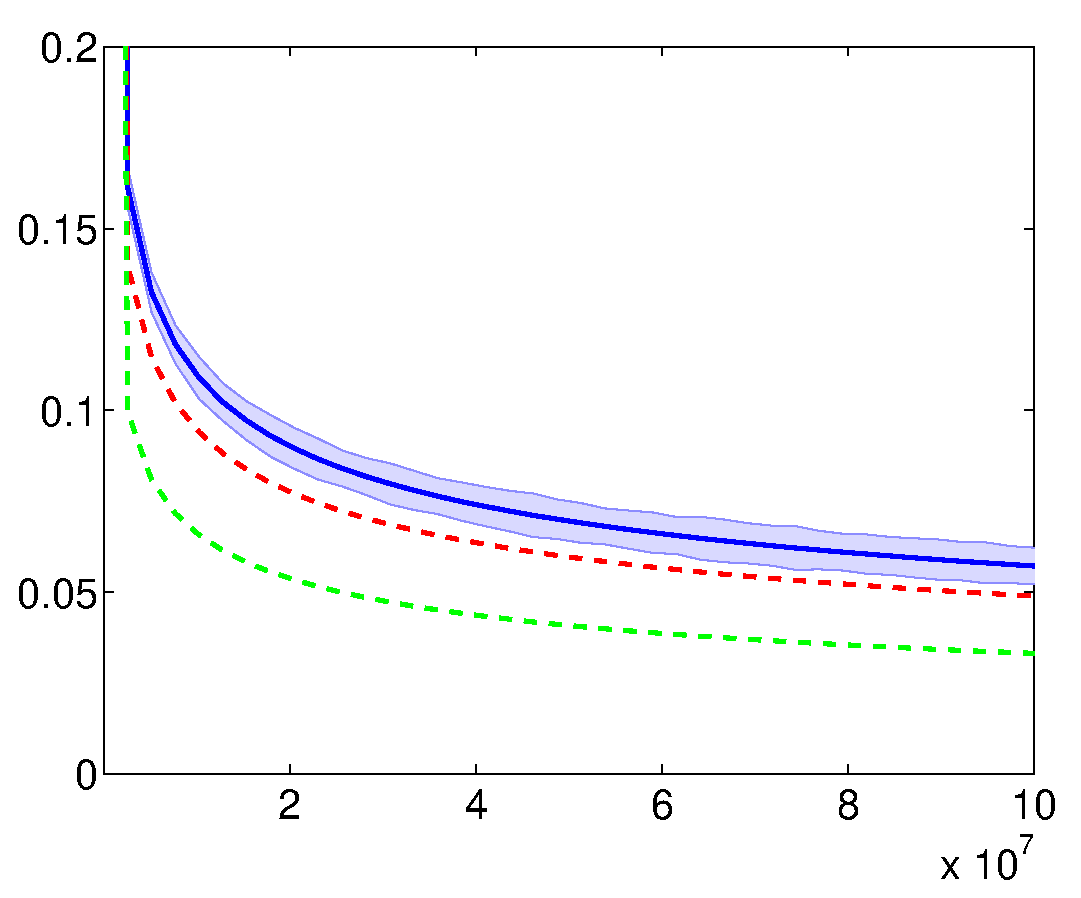
\includegraphics[width=.45\linewidth]{results-rmse/shrodinger-cat-eta9-rmse}\\
Coherent $q_0=3$ &
Schr\"{o}dinger cat $q_0=3$ \\
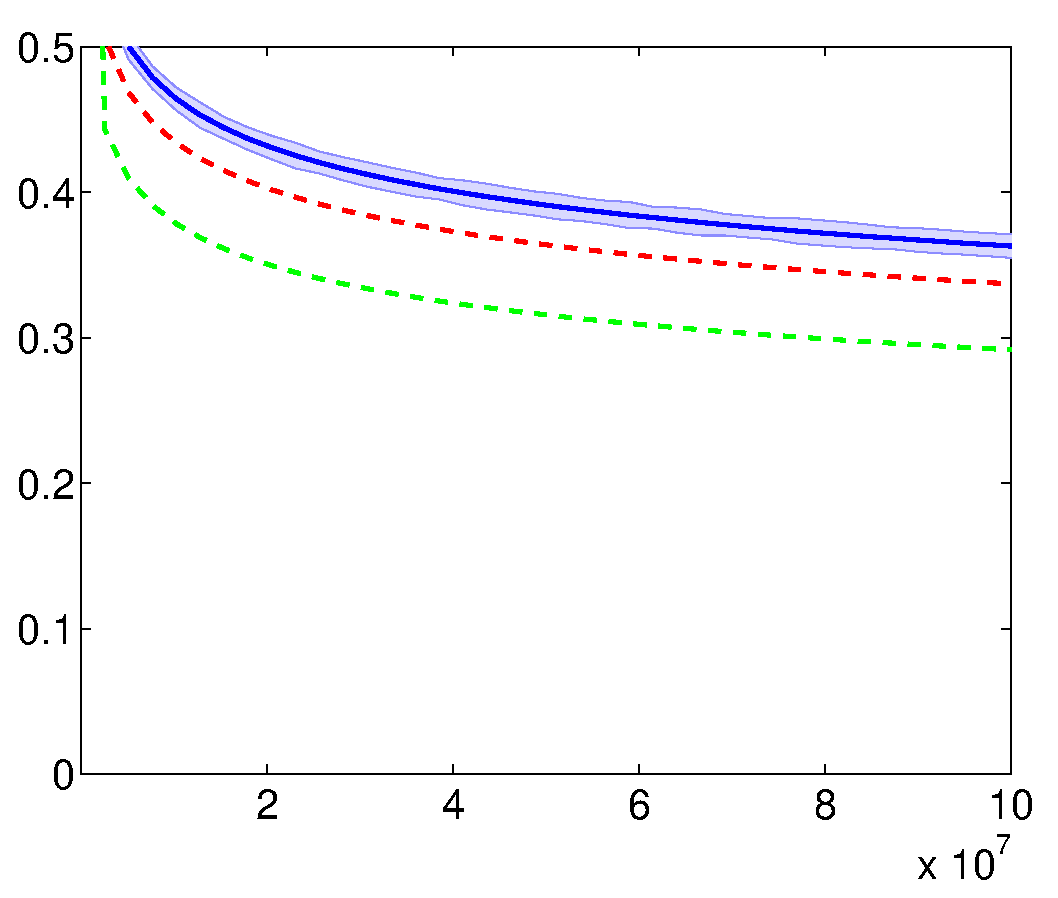
\includegraphics[width=.45\linewidth]{results-rmse/thermal-10-eta9-rmse}& 
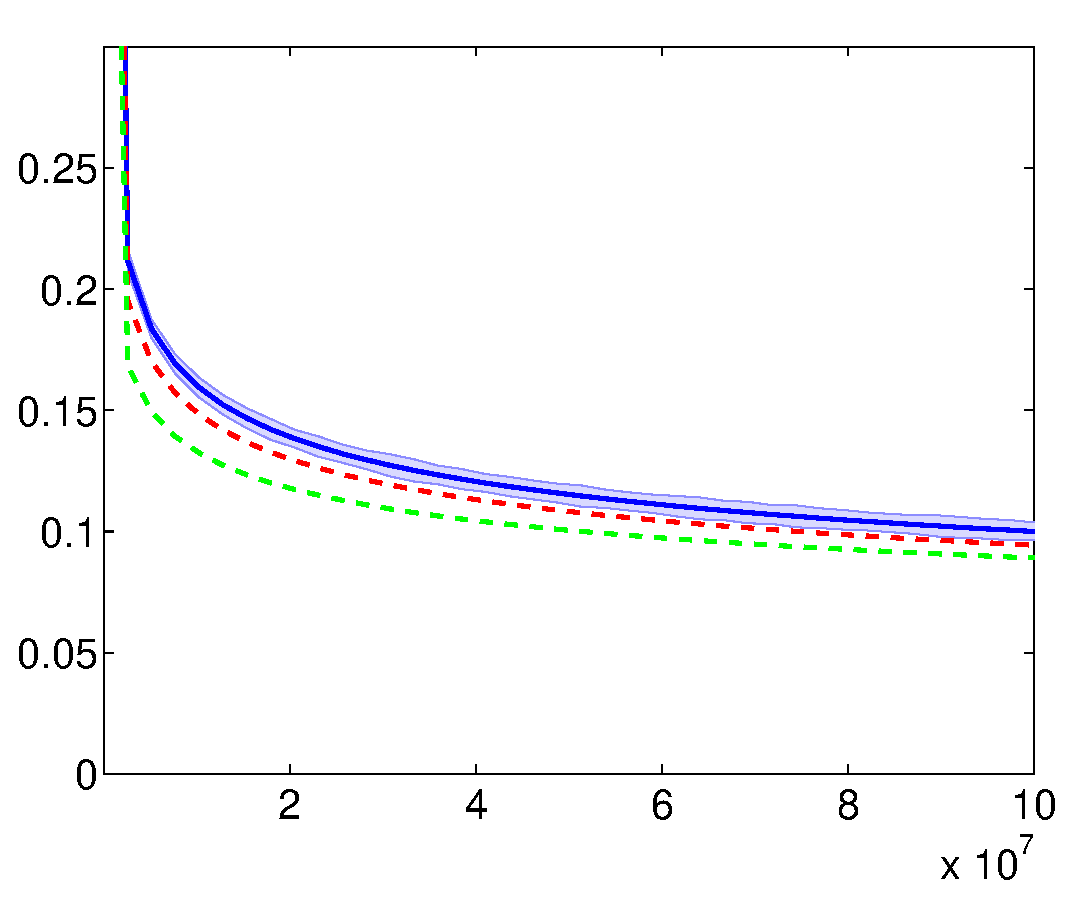
\includegraphics[width=.45\linewidth]{results-rmse/thermal-25-eta9-rmse} \\
Thermal $\beta=1/10$  & Thermal $\beta=1/4$
\end{tabular}
\caption{ % 
	Blue curve: Evolution of $\mathbb{E}( \text{RMSE}(n) )$ as a function of $n$ for $\eta=0.9$, $\varepsilon=1$.
	The blue shaded area represent the confidence interval 
	at $\pm 3$ times the standard deviation of RMSE$(n)$.
	Red (reps. green) curve: evolution of $\mathbb{E}( \text{RMSE}(n) )$ obtained when replacing the threshold $t_{j,k}$ by $0.8 t_{j,k}$ (resp. $0.5 t_{j,k}$) in the estimator in~\eqref{rho-seuil}.
}
\label{fig:RMSE}
\end{center}
\end{figure}

We found numerically that the decay of the RMSE with $n$ almost perfectly fits a power-law, which (up to logarithmic factor) is in accordance with the upper-bounds of Corollary~\ref{coro1}. Following this Corollary in the setting $\eta\in(\frac{1}{2},1)$ and $ r=2$,  we fit a power law of the form 
\begin{equation*}
	\mathbb{E}(\text{RMSE}(n)) \approx n^{ -\frac{\tilde B}{2 ( 4 \gamma+\tilde B)} }.
\end{equation*}
We perform a linear regression in a log-log domain to estimate $\tilde B$. 
Table~\ref{tab:B} reports the estimated value of $\tilde B$ we found using this procedure. 

\begin{table}[!h]
\caption{Estimated values of $\tilde B$ when using $\eta=0.9$, $\varepsilon=1$ and $N=30$.}
\label{tab:B}
\begin{center}
\begin{tabular}{|c|c|c|c|}
\hline 
Coherent $q_0=3$ &
Schr\"{o}dinger cat $q_0=3$ &
Thermal $\beta=1/10$ & 
Thermal $\beta=1/4$ \\ \hline
$\tilde B \approx 0.174$ &
$\tilde B \approx 0.227$ &
$\tilde B \approx 0.037$ & 
$\tilde B \approx 0.082$ \\\hline
\end{tabular}
\end{center}
\end{table}







%%%%%%%%%%%%%%%%%%%%%%%%%
\section{Proof of Theorem \ref{thm.oracle}}
\label{sec.proofs}
\noindent\\
%%%%%%%%%%%%%%%%%%%%%%%%%
%%%%%%%%%

The proof follow the main lines of \cite{Alquier2008a,Alquier2008b}. First, we
need
a set of preliminary lemmas.

%%%%%%%%%%%%%%%%%%
\subsection{Some preliminary results}
\noindent\\
%%%%%%%%%


\begin{lemma}
                \label{lem.deviation}
                For some fixed $\varepsilon\in(0,1)$, let us define the set
                $$
                \Omega_{\varepsilon}\deq \left\{ \forall (j,k)\in J(N),\quad
\left|\hat{\rho}^\eta_{j,k} - \rho_{j,k} \right| \leq t_{j,k} \right\},
                $$
                where the $( t_{j,k})_{j,k}$ are defined in \eqref{tjk} and the
set $J(N)$ is defined in \eqref{eqJ}. Then we have
                $$P(\Omega_{\varepsilon})\geq1-\varepsilon.$$
\end{lemma}

\begin{proof} 
Lemma~\ref{lem.deviation} is proved by using  Hoeffding's inequality. In
this aim, we have to first notice
$$E_\rho[\hat{\rho}^\eta_{j,k}]=\rho_{j,k}.$$
Indeed, by using \eqref{Gjk} , \eqref{fourierproun}, \eqref{eq:patterneta} and
\eqref{rhojk}, we have 
\begin{align*}
        E_\rho[\hat{\rho}^\eta_{j,k}] &=
        E_\rho[G_{j,k}(\frac{Y}{\sqrt\eta},\Phi)] =
        E_\rho[f_{j,k}^{\eta}(\frac{Y}{\sqrt\eta})e^{-i(j-k)\Phi}]
         \\
        & =\frac{1}{\pi}\int_0^\pi e^{-i(j-k)\phi}\int
        f_{j,k}^{\eta}(y)\sqrt{\eta}p_\rho^\eta(y\sqrt{\eta}|\phi)dy
        d\phi\\
        &= \frac{1}{\pi}\int_0^\pi e^{-i(j-k)\phi}\frac{1}{2\pi}\int
        \widetilde{f}_{j,k}^{\eta}(t)
        \mathcal{F}_1[\sqrt{\eta}p_\rho^\eta(\cdot\sqrt{\eta}|\phi)](t)dt
        d\phi\\
        &= \frac{1}{\pi} \int_0^\pi e^{-i(j-k)\phi} \frac{1}{2\pi}
        \int \widetilde{f}_{j,k}(t) e^{\gamma
          t^2} \mathcal{F}_1[p_\rho(\cdot|\phi)](t)
        \widetilde{N}^\eta(t) dt d\phi\\
                &= \frac{1}{\pi}    \int_0^\pi   \int  e^{-i(j-k)\phi} 
    f_{j,k}(x) p_\rho(x|\phi)dx d\phi=\rho_{j,k}.
\end{align*} 
 Moreover, we easily get from the definition of $G_{j,k}$ in \eqref{Gjk} that
for all $\ell=1\cdots,n$ and  $\forall (j,k)\in J(N)$
   $$ - \|f_{j,k}^{\eta}\|_{\infty} \leq
G_{j,k}\paren{\frac{Y_\ell}{\sqrt\eta},\Phi_\ell}\leq\|f_{j,k}^{\eta}\|_{\infty}
.
   $$
Then, for 
   $$
   t_{j,k} =
\|f_{j,k}^{\eta}\|_{\infty}\sqrt{\frac{2\log\left(\frac{N(N+1)}{\varepsilon}
\right)}{n}}%\,\, \forall j,k\text{ s.t. }0\leq j+k \leq N-1,
  $$
  and according to Hoeffding's inequality,
\begin{multline*}
         P \left( \left|   \hat{\rho}^\eta_{j,k} - \rho_{j,k} \right| \geq
t_{j,k}   \right) 
       \\
       = P \left\{ \left| \frac{1}{n}\sum_{\ell=1}^{n}  \left[
G_{j,k}\paren{\frac{Y_\ell}{\sqrt\eta},\Phi_\ell}
        - E \left(G_{j,k}\paren{\frac{Y_\ell}{\sqrt\eta},\Phi_\ell}\right)
\right]\right| \geq t_{j,k}    \right\}
\\
\leq 2 \exp\left[ - \frac{nt_{j,k}^{2}}{2
\|f_{j,k}^{\eta}\|_{\infty}^{2}}\right]
          = \frac{2 \varepsilon}{N(N+1)} .
\end{multline*}
By the classical union bound argument:
 \begin{align*}
          P \left(\Omega_{\varepsilon}^c  \right) 
         & \leq \sum_{ (j,k)\in J(N)} P \left( \left|  \hat{\rho}^\eta_{j,k} -
\rho_{j,k}
         \right| \geq t_{j,k}    \right)\leq \sum_{ (j,k)\in J(N)} \frac{2
\varepsilon}{N(N+1)}\leq \varepsilon .
\end{align*}
\end{proof}


\begin{lemma}
           \label{lem.projection}
            For some fixed $\varepsilon\in(0,1)$ and $\forall(j,k)\in J(N)$,
with $J(N)$ defined in \eqref{eqJ}, we define the set
            $$
             R_{j,k}^{\varepsilon}\deq \left\{ \nu \text{ density matrix},
|\nu_{j,k} - \hat{\rho}^\eta_{j,k}| \leq t_{j,k} \right\},
            $$
            where the $( t_{j,k})_{j,k}$ are defined in \eqref{tjk}. Then, on
the event $\Omega_{\varepsilon}$ defined in Lemma~\ref{lem.deviation} and
$\forall (j,k)\in J(N)$
          \begin{enumerate}
             \item $\rho\in R_{j,k}^{\varepsilon}$.
             \item $R_{j,k}^{\varepsilon}$ is closed and convex set.
             \item For $\Pi_{j,k}^{\varepsilon} $ the orthogonal projection onto
$ R_{j,k}^{\varepsilon}$ and for any density matrix $\nu$,
                 \begin{equation}
                   \label{eq.improv}
                   \left\|\rho - \Pi_{j,k}^{\varepsilon}(\nu) \right\|^{2}_{2} 
\leq \left\|\rho - \nu \right\|^{2}_{2} .
                 \end{equation}
         \end{enumerate}
\end{lemma}

\begin{proof}
The first point is just a consequence of Lemma~\ref{lem.deviation}. The second
point  comes from the definition of $R_{j,k}^{\varepsilon}$. \\
Moreover, it is well known that for any closed and convex set $\mathcal{C}$, if
$\Pi_{\mathcal{C}}$ is the orthogonal projection on $\mathcal{C}$, the following
property holds:
$$ 
\forall x\in\mathcal{C} ,\forall y,\quad \|\Pi_{\mathcal{C}}(y) - x \|_2 \leq
\|y-x\|_2 . 
$$
This concludes the proof of the third point.
\end{proof}

\begin{lemma}
          \label{lem.formule}
          For $\varepsilon\in(0,1)$, any fixed $(j,k)\in J(N)$, with $J(N)$
defined in \eqref{eqJ}, and any density matrix $\nu$, we denote by $\nu'$ the
projection of $\nu$ into $R_{j,k}^{\varepsilon}$,
          $$
          \nu' \deq \Pi_{j,k}^{\varepsilon}(\nu)=[\nu'_{\ell,m}]_{\ell,m},
          $$
          with $R_{j,k}^{\varepsilon}$ defined in Lemma~\ref{lem.projection}.
Then, the entries $\nu'_{\ell,m}$  of $\nu'$ are equal to
          $$
          \nu'_{\ell,m} =\left\{
          \begin{array}{l}
          \nu_{j,k} + {\rm sgn} (\hat{\rho}_{j,k}^{\eta} -
\nu_{j,k})\left(\left|\hat{\rho}_{j,k}^{\eta} -
\nu_{j,k}\right|-t_{j,k}\right)_{+},\text{ if } (\ell,m)=(j,k),\\\\
          \nu_{\ell,m}, \text{ otherwise.}
           \end{array}\right.
           $$
\end{lemma}

\begin{center}
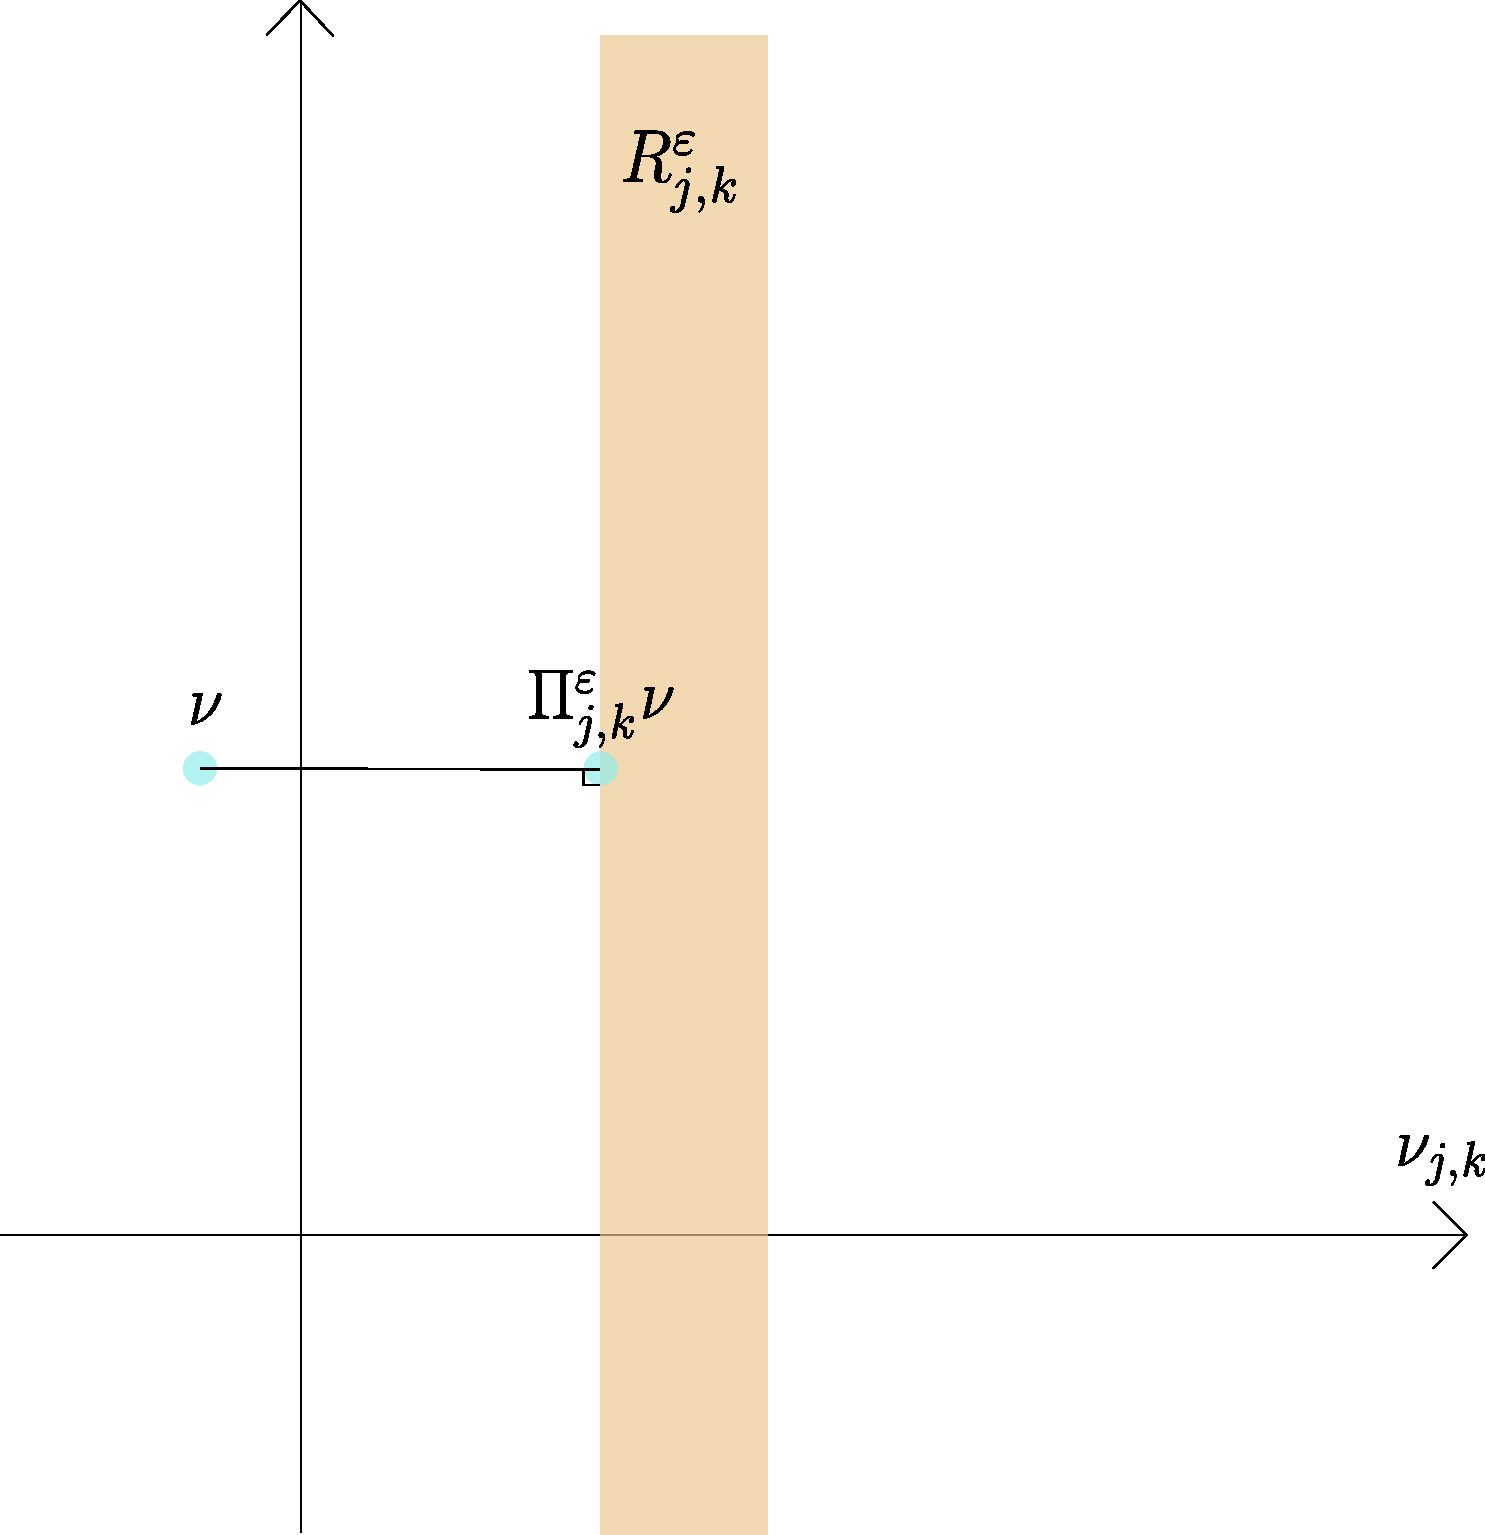
\includegraphics[width=8cm]{dessin.pdf}
\end{center}

\begin{proof}
The projection $\nu'$ of $\nu$ into $R_{j,k}^{\varepsilon}$ satisfies
      $$
      \nu' = \arg\min_{x\in R^{\varepsilon}_{j,k}} \|\nu - x\|_{2}^{2}  =
\arg\min_{x\in R^{\varepsilon}_{j,k}} \sum_{\ell,m=0}^{\infty} \left|x_{\ell,m}
- \nu_{\ell,m} \right|^{2} .
      $$
     As the constraint $x\in R^{\varepsilon}_{j,k}$ is only a constraint on
$x_{j,k}$, it is clear that for $(\ell,m)\neq(j,k)$ the minimum is reached for
$x_{j,k}=\nu_{j,k}$. Finally,
    $$
    \nu'_{j,k} = \arg\min_{x_{j,k}:\,|x_{j,k} - \hat{\rho}_{j,k}^{\eta}|\leq
t_{j,k} } (\nu_{j,k} - x_{j,k})^{2}. 
    $$
The solution $\nu'_{j,k}$ is obvious:
             \begin{align*}
                \nu'_{j,k} & = \left\{\begin{array}{l l}
                  \hat{\rho}_{j,k}^{\eta} - t_{j,k} & \text{ if } \nu_{j,k} <
\hat{\rho}_{j,k}^{\eta} - t_{j,k},\\\\
                  \nu_{j,k} & \text{ if } \hat{\rho}_{j,k}^{\eta} - t_{j,k} \leq
\nu_{j,k} \leq  \hat{\rho}_{j,k}^{\eta} + t_{j,k},\\\\
                  \hat{\rho}_{j,k}^{\eta} + t_{j,k} & \text{ if } \nu_{j,k} >
\hat{\rho}_{j,k}^{\eta} + t_{j,k}
                   \end{array}\right.\\
                & = \nu_{j,k} + {\rm sgn} (\hat{\rho}_{j,k}^{\eta} - \nu_{j,k})
                 \left(\left|\hat{\rho}_{j,k}^{\eta} -
\nu_{j,k}\right|-t_{j,k}\right)_{+}.
            \end{align*}
where the function ${\rm sgn}(\cdot)$ is as defined in \eqref{sgn} and $(\cdot)_+$ is
defined in \eqref{qte+}.
\end{proof}





\begin{dfn} 
    For $m>0$ an integer, let 
    $$
    I \deq \{(j_1,k_1),\dots,(j_m,k_m)\}\subseteq J(N)
    $$
    be a set of indices, where $J(N)$ is the set defined in \eqref{eqJ}. % such
that $\forall \ell\neq i$, $(j_\ell,k_\ell)\neq (j_i,k_i)$. 
      For $\varepsilon\in(0,1)$ and for any density matrix $\nu$, we denote by
$\Pi_{I}^{\varepsilon}(\nu)$ the successive projections of $\nu$ into spaces
$\left(R_{j_i,k_i}^{\varepsilon}\right)_{j_i,k_i}$, i.e.
      $$
       \Pi_{I}^{\varepsilon}(\nu)\deq\Pi_{j_m,k_m}^{\varepsilon}
\Pi_{j_{m-1},k_{m-1}}^{\varepsilon} \ldots \Pi_{j_2,k_2}^{\varepsilon}
\Pi_{j_1,k_1}^{\varepsilon}( \nu ).
     $$
  \end{dfn}
Note that  for any set of indices $I$ and from Lemma~\ref{lem.formule}, the
application of the successive projections $\Pi_{I}^{\varepsilon}$ to a density
matrix $\nu$
does not depend on the order of the successive projections.


\begin{lemma}
         \label{lem.estimator}
         For $\varepsilon\in(0,1)$,  for $J(N)$ defined in \eqref{eqJ} and for
$\tilde{\rho}^{\eta}$ defined in \eqref{rho-seuil}, we have
          $$
          \tilde{\rho}^\eta = \Pi_{J(N)}^{\varepsilon}({\bf 0}),
          $$
          where ${\bf 0}$ is the zero-infinite matrix.
\end{lemma}

\begin{proof}
         This is obvious from the definition of $\tilde{\rho}^\eta$ and from
Lemma~\ref{lem.formule} applied to $\nu={\bf 0}$.
\end{proof}




%%%%%%%%%%%%%%%%%%%%%%%%%
\subsection{Proof of Theorem \ref{thm.oracle}}
\noindent\\
%%%%%%%%%%%%%%%%%%%%%%%%%

\begin{proof}%[

For $J(N)$ the set of indices defined in \eqref{eqJ}, let $I$ be a subset of
$J(N)$, $I\subseteq J(N)$. For a fixed $\varepsilon\in(0,1)$, we have by
Lemma~\ref{lem.estimator} and by successive applications of  the
inequality\eqref{eq.improv} to all pair of indices $(j,k)\notin I$

 \begin{align}
 \label{eq1}
             \| \tilde{\rho}^\eta-\rho \|_{2}^{2}& = \| \Pi_{J }^{\varepsilon}(
{ \bf 0} )-\rho \|_{2}^{2}  \leq \| \Pi_{I }^{\varepsilon}( {\bf 0} )-\rho
\|_{2}^{2}.
  \end{align}
%
Moreover, from Lemma~\ref{lem.formule} applied to $\nu={\bf 0}$, we get 
$$
(\Pi_{I}^{\varepsilon} ({\bf 0}))_{j,k}= \left\{
\begin{array}{l l} {\rm sgn} (\hat{\rho}_{j,k}^{\eta})
\left(|\hat{\rho}_{j,k}^{\eta}|- t_{j,k} \right)_{+} & \text{ if } (j,k)\in I,\\
0 & \text{ otherwise.}\end{array}\right.
$$
Therefore, from \eqref{eq1} we get
             \begin{align}
             \label{eq2}
               \| \tilde{\rho}^\eta-\rho \|_{2}^{2}
             & \leq \sum_{j,k=0}^{\infty} \left[\rho_{j,k} -
(\Pi_{I}^{\varepsilon} ({\bf 0}))_{j,k} \right]^{2}\nonumber\\
             & = \sum_{(j,k)\in I} \left[\rho_{j,k} -  {\rm sgn}
(\hat{\rho}_{j,k}^{\eta})\left(|\hat{\rho}_{j,k}^{\eta}|- t_{j,k} \right)_{+}
\right]^{2} + \sum_{(j,k)\notin I} \rho_{j,k}^{2}\nonumber\\
             &\deq \sum_{(j,k)\in I} \left[A_{j,k}\right]^{2} +
\sum_{(j,k)\notin I} \rho_{j,k}^{2},
             \end{align}
where
\begin{eqnarray*}
A_{j,k}&=&\rho_{j,k} -  {\rm sgn}
(\hat{\rho}_{j,k}^{\eta})\left(|\hat{\rho}_{j,k}^{\eta}|- t_{j,k} \right)_{+}\\
&=& \left\{ \begin{array}{ccc}
                       \rho_{j,k}, & \text{if  }|\hat{\rho}_{j,k}^{\eta}|\leq
t_{j,k},\\\\
                          \rho_{j,k}-\hat{\rho}^\eta_{j,k}+ t_{j,k},& \text{if 
}\hat{\rho}_{j,k}^{\eta}> t_{j,k},\\\\
                          \rho_{j,k}-\hat{\rho}^\eta_{j,k} - t_{j,k},&  \text{if
 }\hat{\rho}_{j,k}^{\eta}<t_{j,k}.
                             \end{array} \right.
\end{eqnarray*}
Moreover
\begin{eqnarray*}
A_{j,k}\leq|A_{j,k}|& \leq & \left\{ \begin{array}{ccc}
                     \left|\hat{\rho}^\eta_{j,k} - \rho_{j,k} \right|
+|\hat{\rho}_{j,k}^{\eta}|, & \text{if  }|\hat{\rho}_{j,k}^{\eta}|\leq
t_{j,k},\\\\
                      \left|\hat{\rho}^\eta_{j,k} - \rho_{j,k} \right|+
t_{j,k},& \text{if  }\hat{\rho}_{j,k}^{\eta}> t_{j,k},\\\\
                      \left|\hat{\rho}^\eta_{j,k} - \rho_{j,k} \right|+
t_{j,k},&  \text{if  }\hat{\rho}_{j,k}^{\eta}<t_{j,k},
                             \end{array} \right.\\
                             &\leq& \left|\hat{\rho}^\eta_{j,k} - \rho_{j,k}
\right|+ t_{j,k}.
\end{eqnarray*}

For any $(j,k)\in I$ and on the event $\Omega_{\varepsilon}$  defined in
Lemma~\ref{lem.deviation}, it holds
$$
\left|\hat{\rho}^\eta_{j,k} - \rho_{j,k} \right| \leq t_{j,k}.
$$
Therefore from \eqref{eq2} 
              \begin{align*}
             %\label{eq2}            
               \| \tilde{\rho}^\eta-\rho \|_{2}^{2}& \leq \sum_{(j,k)\in I} ( 2
t_{j,k} )^{2} + \sum_{(j,k)\notin I} \rho_{j,k}^{2}.
             \end{align*}
We conclude the proof by taking the infimum over the set $I\subseteq J(N)$.
\end{proof}




\bibliographystyle{alpha}
\bibliography{biblio}

\end{document}
